\documentclass[a4paper,12px]{article}
\usepackage{graphicx}
\usepackage[english]{babel}
\usepackage{fancyhdr}
\usepackage{lastpage}
\usepackage{xifthen}
\usepackage[linesnumberedhidden, titlenotnumbered]{algorithm2e}
\usepackage{lipsum}
\usepackage{hyperref}
\usepackage{array}
\usepackage{tabularx}
\usepackage{caption}
\usepackage{amsfonts}
\usepackage{amssymb}
\usepackage{amsmath}
\usepackage{placeins}
\usepackage{enumitem}

\usepackage{minted}
\usepackage{listings}
\usepackage{dsfont}
\usepackage{units}

\pagestyle{fancy}
\lhead{
\includegraphics[width=7cm]{logoUvA}}
\rhead{\footnotesize \textsc {Report\\ \opdracht}}
\lfoot
{%
    \footnotesize \studentA
    \ifthenelse{\isundefined{\studentB}}{}{\\ \studentB}
    \ifthenelse{\isundefined{\studentC}}{}{\\ \studentC}
    \ifthenelse{\isundefined{\studentD}}{}{\\ \studentD}
    \ifthenelse{\isundefined{\studentE}}{}{\\ \studentE}
}
\cfoot{}
\rfoot{\small \textsc {Page \thepage\ of \pageref{LastPage}}}
\renewcommand{\footrulewidth}{0.5pt}

\fancypagestyle{firststyle}
{%
    \fancyhf{}
    \renewcommand{\headrulewidth}{0pt}
    \chead{
\includegraphics[width=7cm]{logoUvA}}
    \rfoot{\small \textsc {Page \thepage\ of \pageref{LastPage}}}
}

\setlength{\topmargin}{-0.3in}
\setlength{\textheight}{630pt}
\setlength{\headsep}{40pt}
\setlength{\parindent}{0pt}

% =================================== DOC INFO ===================================

\newcommand{\opdracht}{Statistisch Redeneren}
\newcommand{\titel}{Lab 2}
\newcommand{\docent}{Rein van de Boomgaard}
\newcommand{\cursus}{Statistisch Redeneren}
\newcommand{\vakcode}{5062STRE6Y}
\newcommand{\datum}{\today}
\newcommand{\studentA}{Maico Timmerman}
\newcommand{\uvanetidA}{10542590}
\newcommand{\studentB}{Tim van Zalingen}
\newcommand{\uvanetidB}{10784012}
% \newcommand{\studentC}{Boudewijn Braams}
\newcommand{\uvanetidC}{10401040}
% \newcommand{\studentD}{Govert Verkes}
\newcommand{\uvanetidD}{10211748}
%\newcommand{\studentE}{Naam student 5}
\newcommand{\uvanetidE}{UvAnetID student 5}

% ===================================  ===================================

\begin{document}
\thispagestyle{firststyle}
\begin{center}
    \textsc{\Large \opdracht}\\[0.2cm]
    \rule{\linewidth}{0.5pt} \\[0.4cm]
    {\huge \bfseries \titel}
    \rule{\linewidth}{0.5pt} \\[0.2cm]
    {\large \datum  \\[0.4cm]}

    \begin{minipage}{0.4\textwidth}
        \begin{flushleft}

            \emph{Students:}\\
            {\studentA \\ {\small \uvanetidA \\[0.2cm]}}
            \ifthenelse{\isundefined{\studentB}}{}{\studentB \\ {\small \uvanetidB \\[0.2cm]}}
        \end{flushleft}
    \end{minipage}
    ~%
    \begin{minipage}{0.4\textwidth}
        \begin{flushright}
            \emph{Lecturer:} \\
            \docent \\[0.2cm]
            \emph{Course:} \\
            \cursus \\[0.2cm]
            % \emph{Student:}\\
            \ifthenelse{\isundefined{\studentC}}{}{\studentC \\ {\small \uvanetidC \\[0.2cm]}}
            \ifthenelse{\isundefined{\studentD}}{}{\studentD \\ {\small \uvanetidD \\[0.2cm]}}
            \ifthenelse{\isundefined{\studentE}}{}{\studentE \\ {\small \uvanetidE \\ [0.2cm]}}
        \end{flushright}
    \end{minipage}\\[1 cm]
\end{center}


% =================================== CONTENTS ===================================

\tableofcontents
\clearpage

% =================================== MAIN TEXT ===================================


\section{Kansrekening 2}

\subsection{Opgave 1}

    %Beschouw de uniforme verdeling op interval $[3,9]$.
    \begin{enumerate}[label=(\alph*)]
        \item De lineaire functie $F(x)$ stijgt op dit interval van 0 naar 1. Dit geeft ons:
        \begin{equation}
            F(x)=\dfrac{x-3}{9-3}=\dfrac{x-3}{6}
        \end{equation}
        Voor $2\leq x \leq 8$.
        \item
            \begin{equation}
                P([-10,3])=F(-10)-F(3)=0-\dfrac{3-3}{6}=0
            \end{equation}
        \item
            \begin{equation}
                P([a,b])=F(a)-F(b)=\dfrac{a-3}{6}-\dfrac{b-3}{6}=\dfrac{a-3-b+3}{6}=\dfrac{a-b}{6}
            \end{equation}
    \end{enumerate}

\subsection{Opgave 2}

    \begin{enumerate}[label=(\alph*)]
        \item $U=\{\text{'kop'},\text{'munt'}\}$
        \item
            \begin{equation}
                P(k)=\binom{n}{k}p^k(1-p)^{n-k}
            \end{equation}
        \item Dit is de binomiale verdeling, met paramters $n$ en $p$.
        \item
            \inputminted{python}{2d.py}
    \end{enumerate}

\subsection{Opgave 3}

    In python met Scipy en Numpy is het mogelijk om statistische functie te
     gebruiken met \textit{scipy.stats}. Hierin zit de normale verdeling als
     \textit{stats.norm}. De kansdichtheidsfunctie in norm is:

    \begin{equation}
        \dfrac{e^{-x^2/2}}{\sqrt{2*\pi}}
    \end{equation}

    We plotten de kansdischtheidsfunctie, de verdelingsfunctie en een histogram
     met 1000 waarden uit de kansdichtheidsfunctie. De code:
    \inputminted{python}{3.py}
    Dit is het resultaat:

    \begin{figure}[!h]
        \centering
        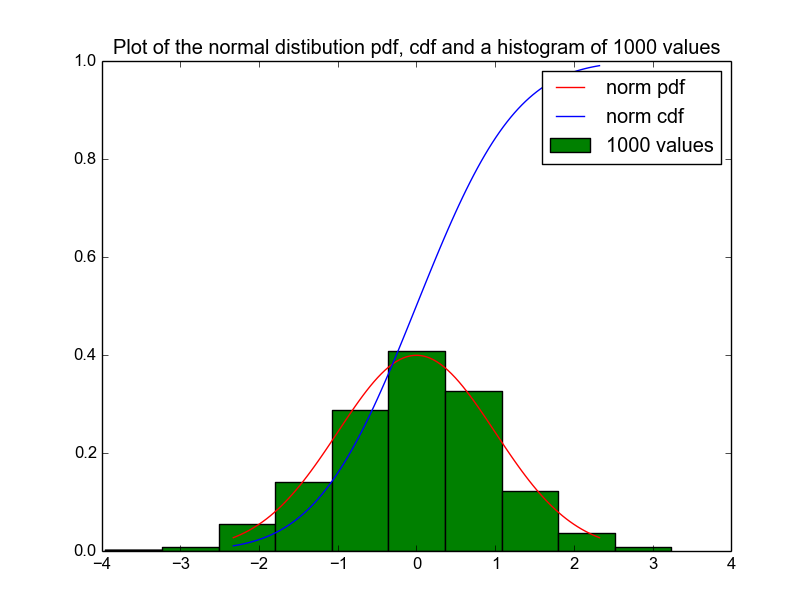
\includegraphics[width=\textwidth]{fig.png}
    \end{figure}
    \FloatBarrier

    De histogram van de 1000 waarden past vrijwel correct in the
    kansdichtheidsfunctie.

\clearpage
\section{Naive Bayes Classifier}

De classificatie of iemand een man of vrouw is, hangt af van de lengte, het
gewicht en de schoenmaat van de persoon. Er wordt vanuit gegaan dat al deze
eigenschappen $\vec x$ normaal verdeeld zijn. Dat wil zeggen dat de kansdichtheidsfunctie
is te beschrijven als een functie van de Gaussian. Om de goede kansdichtheids
functie te berekenen wordt het gemiddelde en de standaarddeviatie berekend.


Gegeven deze eigenschappen, willen we weten wat de kans is dat de data hoort bij
een man of bij een vrouw ($S$). De kans die het grootste is wordt als waarheid
beschouwd.

Volgens de stelling van Bayes geldt:

$$ p(S|\vec x) = \frac{p(S)p(\vec x|S)}{p(\vec x)}$$

Dit willen we oplossen voor $S = man$ en $S = vrouw$.

Omdat voor beide berekeningen geldt dat $p(\vec x)$ hetzelfde is, kunnen we deze
buiten beschouwing laten, dus hoeven we alleen $p(S)p(\vec x|S)$ op te
lossen.

Volgens de chain rule geldt dat kansen die onafhankelijk zijn geschreven worden
als:

$$p(x_l, x_g, x_s|S) = p(x_l|S)p(x_g|S)p(x_s|S)$$

De kansen $p(x_i|S)$ zijn te berekenen met de kansdichtheidsfuncties die we
eerder hebben opgesteld.


$$P(S_m)p(x_l|S_m)p(x_g|S_m)p(x_s|S_m) > P(S_v)p(x_l|S_v)p(x_g|S_v)p(x_s|S_v)$$

Omdat we werken met mannen en vrouwen is de kans theoretisch gezien even groot.
Dus deze laten we ook weg uit de vergelijking. En kunnen we een man
classificeren als volgt:

$$p(x_l|S_m)p(x_g|S_m)p(x_s|S_m) > p(x_l|S_v)p(x_g|S_v)p(x_s|S_v)$$

In onze programma hebben we de data van 2014 gebruikt als data om de
kansdichtheidsfuncties te berekenen en de data van 2016 als test en vice versa.

Resultaten hiervan zijn de zien in de volgende figuren en tabellen. Helaas is
de trainingsdata voor vrouwen erg weinig, waardoor het moeilijker wordt om met
zekerheid te zeggen over de kans dat iemand een vrouw is.

\begin{figure}[h!]
    \centering
    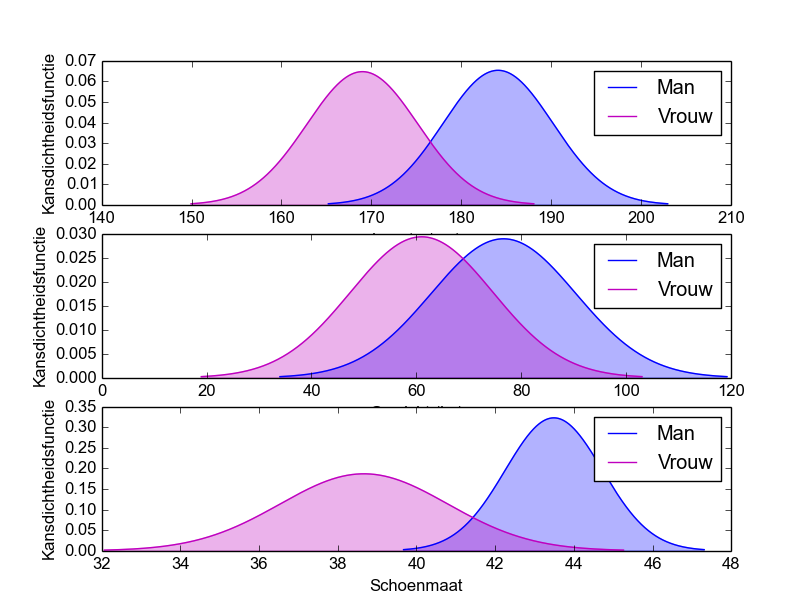
\includegraphics[width=0.8\textwidth]{sex14.png}
    \caption{De kansdichtheidsfunctie met trainingsdata van 2014}
    \label{fig:sex_image}
\end{figure}
\FloatBarrier

\begin{table}[h]
\begin{tabular}{l|ll}
                      & man & vrouw \\\hline
Geclassificeerd man   & 36 & 4 \\
Geclassificeerd vrouw & 4  & 5 \\
\end{tabular}
\caption{De confusion matrix met trainingsdata van 2014 en testdata van 2016}
\end{table}

\begin{figure}[h!]
    \centering
    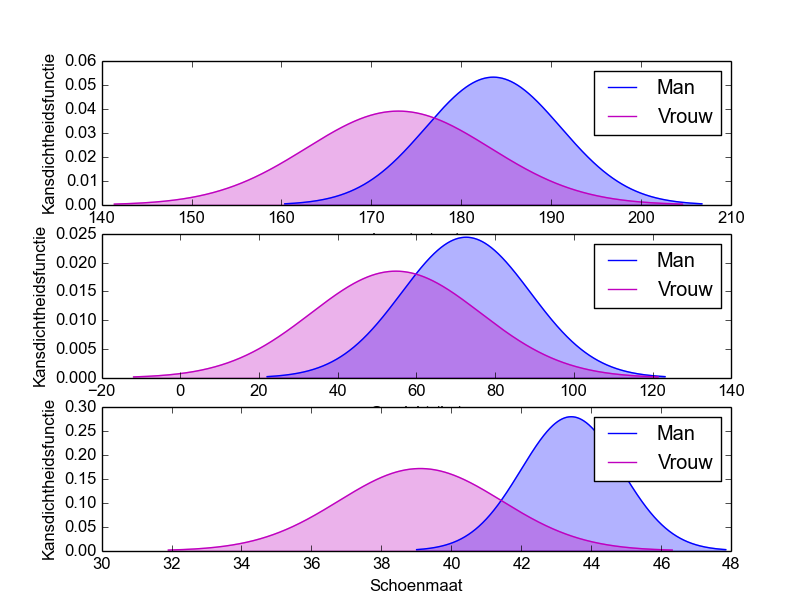
\includegraphics[width=0.8\textwidth]{sex16.png}
    \caption{De kansdichtheidsfunctie met trainingsdata van 2016}
    \label{fig:sex_image}
\end{figure}
\FloatBarrier

\begin{table}[h]
\begin{tabular}{l|ll}
                      & man & vrouw \\\hline
Geclassificeerd man   & 26 & 1 \\
Geclassificeerd vrouw & 2  & 5 \\
\end{tabular}
\caption{De matrix met trainingsdata van 2016 en testdata van 2014}
\end{table}


% =================================== REFERENCES ===================================

%\clearpage
% \bibliographystyle{apalike}
% \bibliography{report}

\end{document}
